% Created 2018-11-23 Fri 13:49
% Intended LaTeX compiler: pdflatex
\documentclass[11pt]{article}
\usepackage[utf8]{inputenc}
\usepackage[T1]{fontenc}
\usepackage{graphicx}
\usepackage{grffile}
\usepackage{longtable}
\usepackage{wrapfig}
\usepackage{rotating}
\usepackage[normalem]{ulem}
\usepackage{amsmath}
\usepackage{textcomp}
\usepackage{amssymb}
\usepackage{capt-of}
\usepackage{hyperref}
\author{Kyle Cotton}
\date{\today}
\title{}
\hypersetup{
 pdfauthor={Kyle Cotton},
 pdftitle={},
 pdfkeywords={},
 pdfsubject={},
 pdfcreator={Emacs 26.1 (Org mode 9.1.9)}, 
 pdflang={English}}
\begin{document}

\tableofcontents

\section{Inf1-Competition}
\label{sec:org58a3b01}
\subsection{Game of Life}
\label{sec:org3b8b115}
Our team has decided to make an improved version of Conan's Game of Life entirely in Haskell.
The code features both two and three dimensional real time rendering.

\subsection{{\bfseries\sffamily TODO} Images}
\label{sec:orgf5664be}

\begin{center}
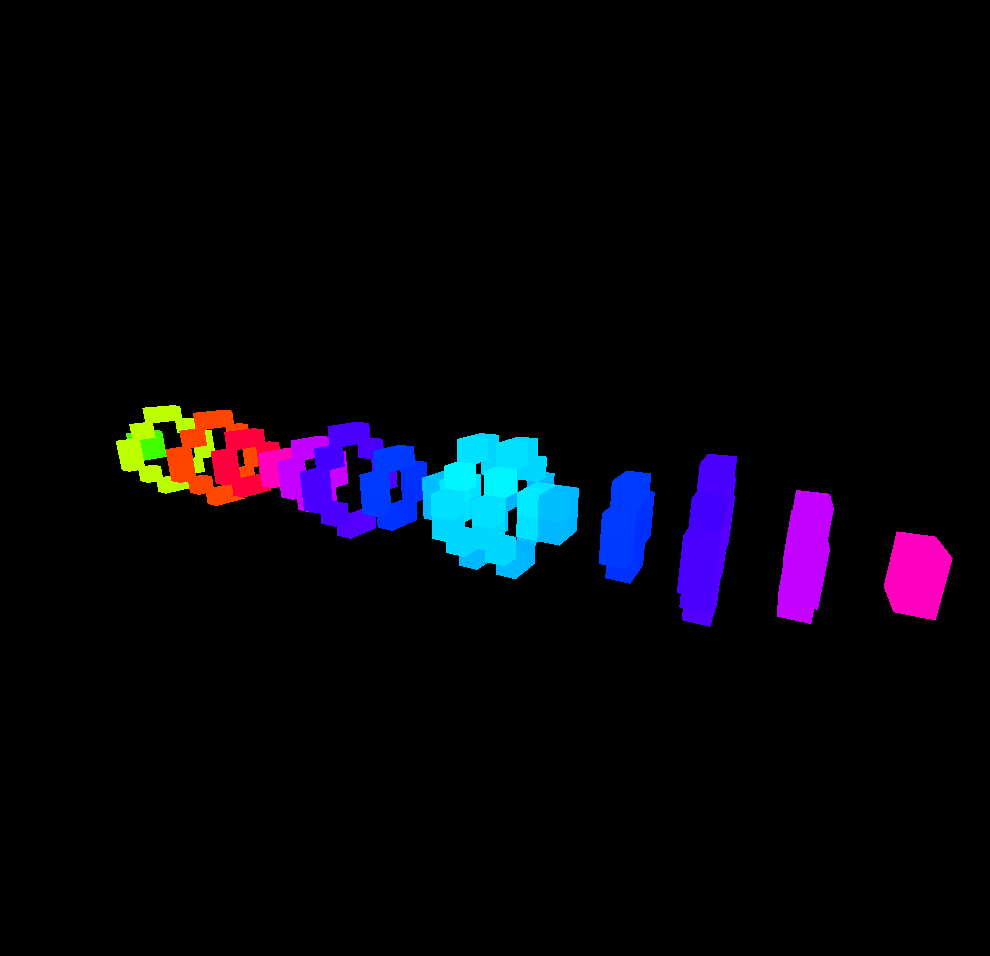
\includegraphics[width=.9\linewidth]{1.png}
\end{center}

\begin{center}
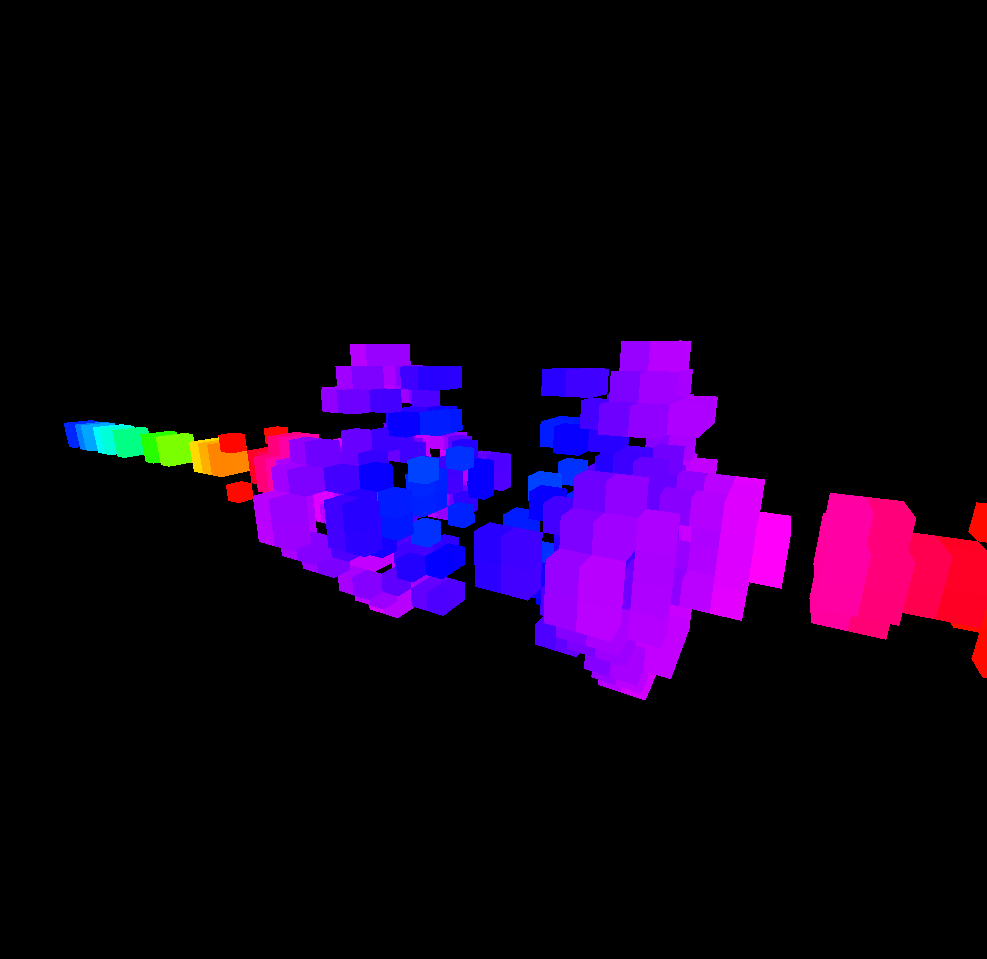
\includegraphics[width=.9\linewidth]{2.png}
\end{center}

\begin{center}
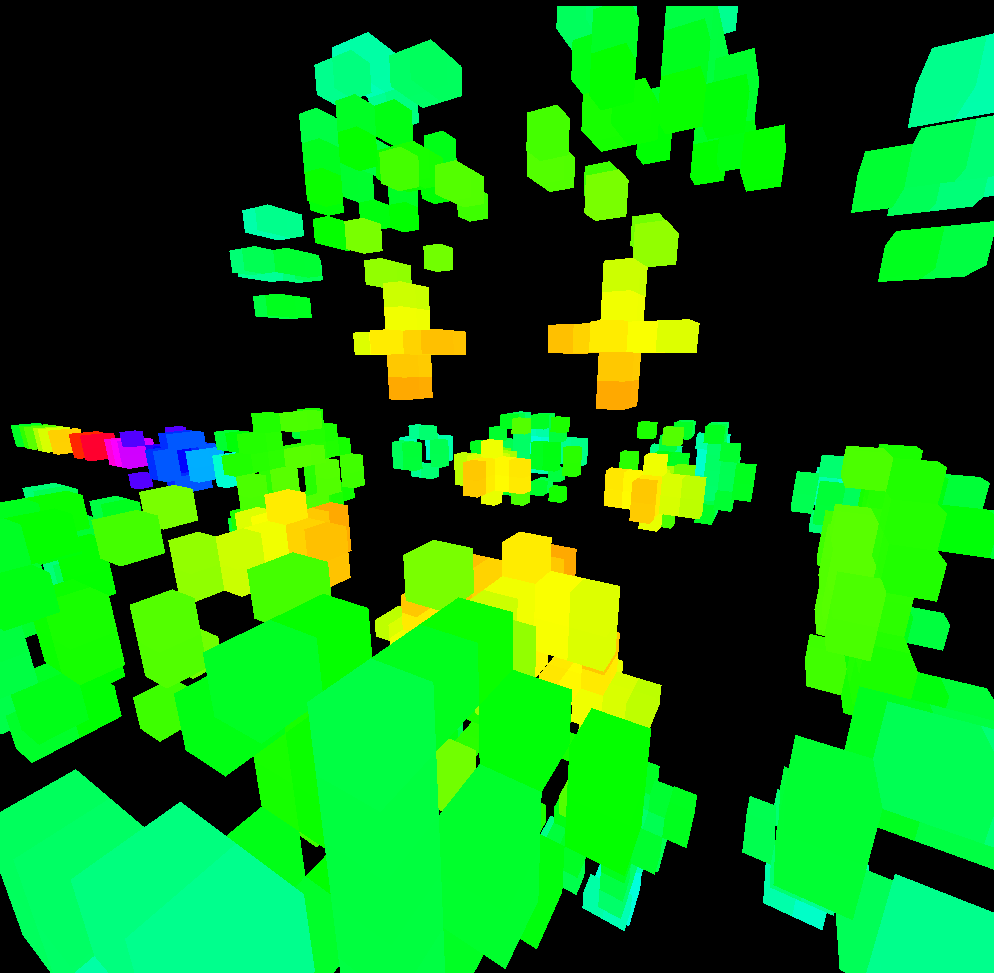
\includegraphics[width=.9\linewidth]{3.png}
\end{center}

\begin{center}
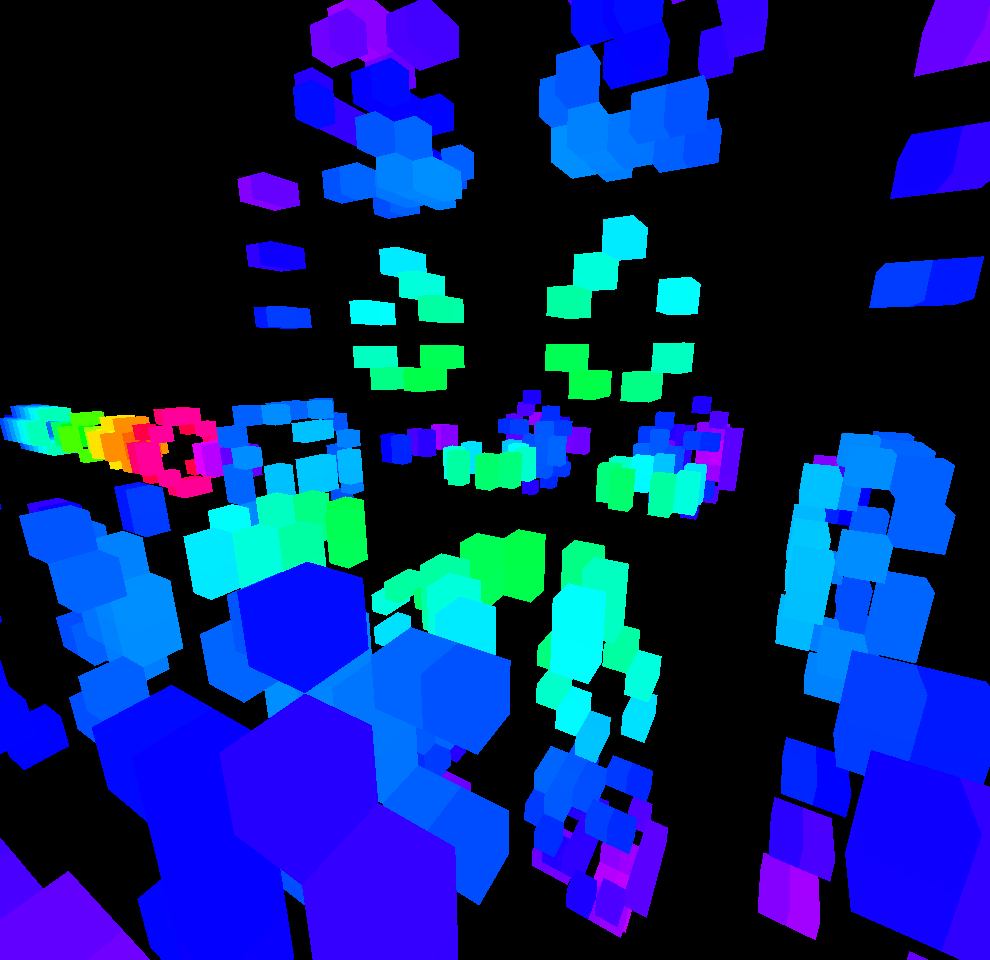
\includegraphics[width=.9\linewidth]{4.png}
\end{center}

\begin{center}
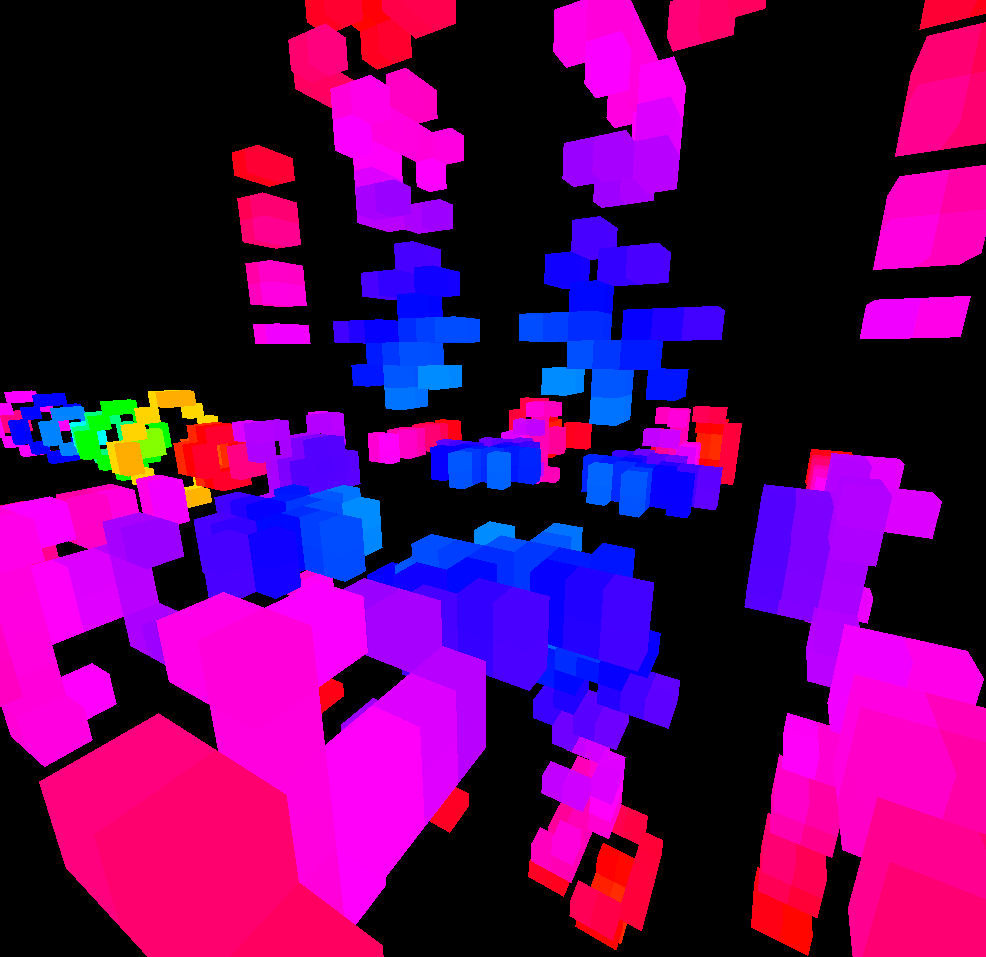
\includegraphics[width=.9\linewidth]{5.png}
\end{center}

\begin{center}
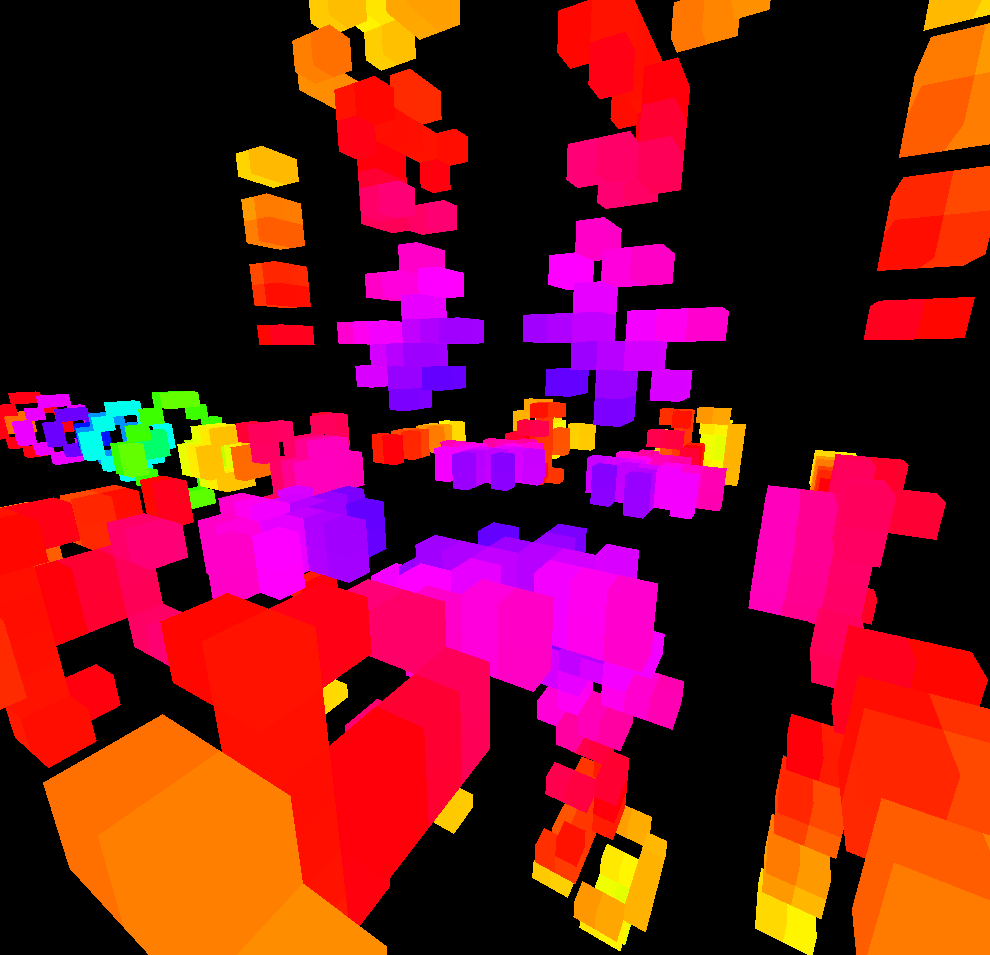
\includegraphics[width=.9\linewidth]{6.png}
\end{center}

\begin{center}
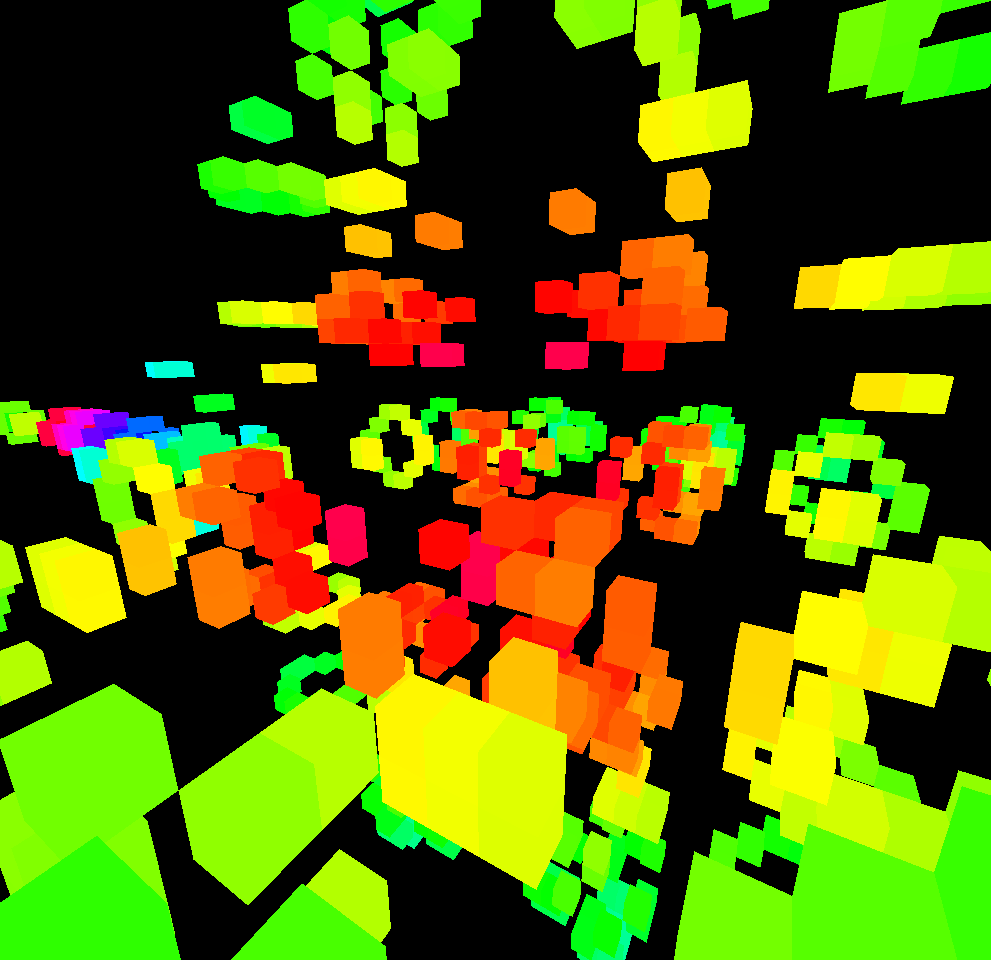
\includegraphics[width=.9\linewidth]{7.png}
\end{center}
\end{document}
